\documentclass[journal, a4paper]{IEEEtran}

\usepackage{graphicx}   
\usepackage{url}        
\usepackage{amssymb}
\usepackage{amsmath}
\usepackage[numbers]{natbib} % Added for compatibility with abbrvnat
\usepackage{hyperref} % Add to your preamble
\usepackage{float}

\usepackage{xcolor}

% Define the \todo command
\newcommand{\todo}[1]{\textcolor{red}{#1}}





% Some useful/example abbreviations for writing math
\newcommand{\argmax}{\operatornamewithlimits{argmax}}
\newcommand{\argmin}{\operatornamewithlimits{argmin}}
\newcommand{\x}{\mathbf{x}}
\newcommand{\y}{\mathbf{y}}
\newcommand{\ypred}{\mathbf{\hat y}}
\newcommand{\yp}{{\hat y}}

\bibliographystyle{abbrvnat}  % Use abbrvnat for references

\begin{document}

\title{Checkmate by learning: A modular Reinforcement Learning approach to chess}
\author{Enzo Pinchon \hspace{3pt} Luis Wiedmann \hspace{3pt} Mathieu Antonopoulos \hspace{3pt} Shashwat Sharma  \hspace{3pt} Yann Baglin-Bunod }
\maketitle

% Write abstract here
\begin{abstract}
    This project presents the development of modular reinforcement learning (RL) algorithms for chess-playing agents, referred to as Chessbots. Our system is designed to provide a simple and flexible framework for defining new agents without the need to rebuild the entire chess logic. It integrates a custom environment using a Python backend, which handles game behavior (via the python-chess library) and model interaction, alongside a lightweight web frontend for visualization and user interaction. The framework supports a wide range of agent architectures, from heuristic-based models to advanced Monte Carlo Tree Search (MCTS) and deep learning-based strategies. Our focus is on implementing modular reinforcement learning algorithms, both with and without deep learning, to explore different approaches to strategic decision-making in chess. The implementation can be found \href{https://github.com/Enzo-py/chess-bot}{here}.
\end{abstract}

% Each section begins with a \section{title} command
\section{Introduction}
\label{sec:intro}

Chess represents an ideal environment for reinforcement learning research due to its complex state space, delayed rewards, and clear win/loss outcomes. The sequential decision-making nature of chess requires agents to balance exploration (trying new moves) and exploitation (leveraging known good moves), a fundamental challenge in RL. We start by establishing baselines with classical techniques such as greedy decision-making algorithms, Monte Carlo Tree Search (MCTS), Alpha-Beta pruning, and Thompson sampling. In addition, we explore deep learning architectures within RL to enhance state evaluation and move probability estimation. 
%Although we are currently experimenting with Convolutional Neural Networks (CNNs)—which, due to their translation equivariance, might not fully capture the nuances of chess—they serve as a promising baseline for more sophisticated models (e.g., Transformers, distillation-based methods, and teacher-student encoder frameworks). 
This is particularly relevant as it addresses key challenges in large state-space problems, delayed reward structures, and complex decision-making, all of which are core difficulties in reinforcement learning.
    
Our project faces several primary challenges. Efficient navigation through the immense state space of chess, which encompasses approximately $10^{43}$ potential positions, requires sophisticated search strategies. Another critical issue is crafting evaluation functions that extend beyond basic material assessment, capturing nuanced positional and strategic subtleties. Traditional chess engines typically employ handcrafted, greedy evaluation methods; however, our goal is to advance beyond these by integrating deep learning techniques.
A fundamental concern in our approach involves effectively balancing exploration and exploitation within search algorithms, including greedy methods and Monte Carlo-based strategies. Furthermore, integrating deep learning architectures into our reinforcement learning framework presents additional complexities. 
%While our initial experiments with convolutional neural networks (CNNs) have established a baseline, their inherent architectural limitations have driven our exploration of alternative models, notably Transformers.
Additionally, the computational intensity required to train deep RL models necessitates optimization strategies to manage resource constraints efficiently. Ensuring modularity within our framework is also paramount, enabling seamless integration and equitable comparisons across diverse methodologies—from simple heuristic and stochastic agents to sophisticated deep RL models.
Lastly, the delayed reward structure inherent in chess, where game outcomes are only revealed upon conclusion, poses significant difficulties in assigning appropriate credit to earlier moves, further complicating our training and evaluation processes.

\section{Background}
\label{sec:background}
\subsection{Related Work}
\noindent Chess has long served as a benchmark for artificial intelligence research. Traditional methods have extensively used the minimax algorithm with alpha-beta pruning, as exemplified by engines like Stockfish \cite{stockfish}, which leverage extensive domain knowledge and sophisticated evaluation functions. Recent advancements, however, have shifted toward pure machine-learning techniques. DeepChess \cite{David_2016} introduced the first end-to-end machine learning method to achieve grandmaster-level performance without relying on prior chess knowledge, using a two-phase training approach involving unsupervised pretraining and a Siamese network for positional comparisons. AlphaZero \cite{silver2018alphazero} further demonstrated the effectiveness of combining Monte Carlo Tree Search (MCTS) with deep neural networks, achieving superhuman performance through self-play alone, without human expertise. Subsequent research has explored employing Mixture of Experts (MoE) alongside MCTS \cite{helfenstein2024checkmatingoneusingmany}, where specialized neural networks target different phases of the game to enhance computational efficiency. Other studies have developed lightweight chess environments with customizable board dimensions, enabling reinforcement learning agents to train through self-play under constrained computational resources \cite{hammersborg2022reinforcementlearningadaptablechess}. Additionally, diverse Q-learning variants, including hierarchical and modular approaches designed to address memory limitations in complex state spaces, have also been explored \cite{8836506}. Our research builds upon these foundational studies, emphasizing implementations optimized for operation within limited computational constraints.




%Chess provides an ideal environment for studying reinforcement learning due to its well-defined rules, clear objectives, and complex state space. In this section, we outline the key concepts and algorithms used in our chess agents.

\subsection{Chess as a Reinforcement Learning Problem}
\noindent Following common reinforcement learning notation, a chess-playing agent can be formalized as a Markov Decision Process (MDP). The state space $\mathcal{S}$ comprises all possible board configurations, including piece positions, castling rights, en passant status, and current player turn information. The action space $\mathcal{A}(s)$ is defined by the set of legal moves available from any given state \( s \in \mathcal{S} \). The transition function $P(s'|s,a)$ is deterministic; given any state-action pair $(s, a)$, the resulting state $s'$ is always uniquely determined, with no uncertainty involved. Chess also features a typically sparse reward function $R(s, a, s')$, which assigns significant feedback primarily at the end of each game, corresponding to a win, loss, or draw. The agent’s behavior is guided by a policy $\pi(a|s)$, which defines the probability distribution of selecting action $a$ in a given state $s$. The goal is to learn a policy $\pi^*$ that maximizes the expected cumulative reward, which in chess corresponds to maximizing the probability of winning.


\subsection{Key Algorithms}
\noindent \textbf{Monte Carlo Tree Search (MCTS): } 
MCTS constructs a search tree incrementally through repeated simulations, carefully balancing the trade-off between exploring new moves and exploiting known successful moves. The algorithm proceeds in four main steps: 
\begin{enumerate}
    \item \textit{Selection}, where it traverses the current search tree from the root using a selection policy, commonly the Upper Confidence Bound (UCB1), until a leaf node is reached;
    \item \textit{Expansion}, which adds one or more child nodes to the selected leaf node to explore new possible moves;
    \item \textit{Simulation}, which estimates the potential outcome by performing random playouts starting from the newly added nodes; and
    \item \textit{Backpropagation}, in which results from these simulations are propagated back up the tree, updating each node’s statistics such as visit counts and win rates.
\end{enumerate}
Formally, the UCB1 policy is given by:
\[
\text{UCB1}(n) = \frac{w_n}{v_n} + c \sqrt{\frac{\ln(v_p)}{v_n}}
\]
where \(w_n\) is the number of wins for node \(n\), \(v_n\) is the number of visits to node \(n\), \(v_p\) is the number of visits to the parent node, and \(c\) is a constant balancing exploration and exploitation.

\noindent \textbf{Alpha-Beta Pruning:} 
Alpha-Beta pruning is an optimization technique applied to the minimax algorithm to significantly reduce the number of nodes evaluated in the search tree. It operates by maintaining two key values during the search: alpha ($\alpha$), representing the best already-explored option along the path for the maximizing player, and beta ($\beta$), representing the best option for the minimizing player. If at any point during the search a branch cannot influence the final outcome (because it leads to outcomes no better than previously examined alternatives), it is pruned. Formally, branches are pruned when:
\[
\alpha \geq \beta,
\]
indicating that further exploration of those branches is unnecessary, as they will not impact the final decision.

\noindent \textbf{Deep Neural Networks:}
Deep neural networks, particularly Convolutional Neural Networks (CNNs), have proven effective at detecting spatial patterns in grid-like structures, making them a natural initial choice for modeling chess positions. 
%In our implementation, CNNs serve two main purposes: evaluating board states by predicting the winning probability from a given position and guiding move generation by recommending the best moves. 
%However, CNNs have limitations in capturing positional dependencies due to their inherently local receptive fields and invariance properties, which can be disadvantageous in chess where exact piece positioning is strategically critical.
Additionally, we explored more sophisticated architectures, notably Transformers, which can effectively encode position-specific context through attention mechanisms. Transformers inherently model global interactions between board squares, which should allow them to better capture complex strategic relationships and sequential dependencies in the game.

\subsection{Evaluation Functions}
\noindent Chess evaluation functions typically combine several strategic factors into a single numerical score to assess board positions. Key components include material assessment—assigning standard values to each piece (e.g., pawn = 100, knight = 320, bishop = 330, rook = 500, queen = 900)—as well as piece positioning, recognizing strategic advantages such as knights controlling central squares. Additional considerations involve king safety, accounting for elements like pawn shields, castling, and exposure to attacks; and positional strength, reflecting the importance of optimal placement for each piece type. Other nuances, such as mobility and pawn structure integrity, are also crucial. These diverse factors are combined, potentially with learned weights, resulting in a comprehensive evaluation metric guiding the decision-making process of chess-playing algorithms.

\section{Methodology/Approach}
\label{sec:methodology}
Our approach centers on a modular, flexible framework designed for implementing and systematically comparing diverse chess-playing agents, with an emphasis on reinforcement learning and deep learning methodologies. The framework is organized into two primary components: a \textbf{backend}, developed in Python, responsible for managing the core game logic, AI algorithms, and integration of machine learning models; and a \textbf{frontend}, providing an intuitive interface for interacting with the chess environment, visualizing games, and interpreting results.

\subsection{Agent Architectures}
\noindent Our methodology begins with baseline agents—such as Random AI and Greedy AI—that provide initial performance benchmarks. Building upon these simple approaches, we integrate classical search algorithms like Monte Carlo Tree Search (MCTS), Alpha-Beta pruning, and Thompson sampling, combined with chess-specific heuristics, to systematically evaluate and compare strategic enhancements. Additionally, we incorporate deep neural network models, including Convolutional Neural Networks (CNNs) and transformer-based architectures, for more sophisticated tasks such as board evaluation and move selection.
The following subsections detail the various agents implemented, organized by increasing complexity:

\subsubsection{Primitive Baseline Agents} 
\paragraph{Random AI} This baseline agent selects moves uniformly at random from all available legal moves, serving as a simple reference point for performance comparison.
\paragraph{Greedy AI} This agent evaluates moves based primarily on immediate material gain, incorporating basic positional heuristics such as central control, piece development, and capturing potential. Special moves, including castling and pawn promotion, receive additional bonuses. However, this agent prioritizes short-term tactical advantages over long-term strategic considerations.

\subsubsection{Greedy Exploration AI}
The Greedy Exploration AI extends the Greedy AI by integrating tree search capabilities. Initially, it evaluates moves using the Greedy AI scoring mechanism to select promising candidates. These candidate moves are then explored more deeply through simulations to estimate long-term outcomes. Specifically, the agent considers the top $N$ candidate moves (\texttt{exploration\_size} = 10), conducts multiple simulations per candidate (\texttt{exploration\_sample} = 150), and explores several moves ahead (\texttt{exploration\_depth} = 3). Strategic moves, such as castling, are rewarded, while suboptimal moves, like occupying board edges unnecessarily, incur penalties. The evaluation function incorporates material balance, piece activity, center control, and king safety.

\subsubsection{Monte Carlo Tree Search AI}
Our MCTS agent implements the standard four-phase algorithm (selection, expansion, simulation, and backpropagation), enhanced by several chess-specific optimizations. These include employing the UCB1 formula with a tunable exploration parameter (set at 0.7), move prioritization based on the Most Valuable Victim–Least Valuable Attacker (MVV-LVA) heuristic \cite{1012769}, and weighted random selection during playouts. Additionally, our simulations use comprehensive position evaluations, accounting for material balance and draw conditions. To maintain computational efficiency, we limit simulation depth to 30 moves and allocate a fixed thinking time of 1.0 second per move. After constructing a search tree within the allocated time, the agent selects the move with the highest visit counts and strongest win-rate estimation.

\subsubsection{Alpha-Beta Pruning based methods}
We implement two agents employing Alpha-Beta pruning combined with iterative deepening, inspired from the SunFish and the Stockfish chess engine. The major improvement to performance comes from positional evaluation using piece-square tables, efficient move ordering to enhance pruning effectiveness, and time-limited search via iterative deepening. The evaluation function incorporates material balance, piece mobility, and king safety, without any deep neural-network based evaluation. Like MCTS, this agent requires no pre-training and is ready to play upon implementation.

\subsubsection{Reinforcement Learning Models}
Our exploration extended to reinforcement learning approaches, implementing two value-based learning methods:

\paragraph{Q-Learning} This agent implements tabular Q-learning, a model-free reinforcement learning technique that learns the value of state-action pairs through iterative interaction with the environment. Our implementation maintains a Q-table to store learned values for board states and associated moves, employing an epsilon-greedy strategy to balance exploration and exploitation during training. The agent updates its value estimates using the Q-learning update rule based on immediate rewards and estimated future returns.

\paragraph{TD-Learning} The Temporal Difference learning agent employs a bootstrapping approach, updating value estimates based on the difference between successive predictions. This implementation uses $TD(\lambda)$ with eligibility traces to propagate rewards efficiently through the state history. By learning value functions that predict expected outcomes from chess positions, the TD-learning agent can make decisions without requiring an explicit model of the environment dynamics. The approach demonstrates how reinforcement learning principles can be applied to the complex state space of chess.

\subsubsection{Deep Network-based Models}
We also explored agents and evaluation functions based on deep neural networks, specifically utilizing CNNs and transformers:

\paragraph{CNNScore} This model employs a CNN architecture to evaluate chess positions, predicting the probability of winning from a given board state. The implementation leverages convolutional layers to process the 8x8 board representation and extract meaningful features from the spatial arrangement of chess pieces.

\paragraph{TreeSearchCNN} Combining CNN-based position evaluation with a tree search mechanism, this model first leverages the neural network to identify promising candidate moves. It then conducts deeper simulations to assess each candidate's long-term potential. Important parameters for this agent include selecting the top 5 candidate moves (\texttt{exploration\_size} = 5), exploring 14 moves ahead (\texttt{exploration\_depth} = 14), performing 200 simulations per candidate (\texttt{exploration\_sample} = 200), and applying a temperature parameter of 1.0 to scale move-selection probabilities.

\paragraph{Transformer} This model implements a transformer-based architecture to evaluate chess positions. By utilizing attention mechanisms, the model can capture complex relationships between pieces on the board, providing sophisticated position assessment capabilities beyond spatial patterns.

\paragraph{TreeSearchTransformer} Similar to its CNN counterpart, this model combines transformer-based evaluation with advanced tree search algorithms. The implementation supports various search strategies including alpha-beta pruning to efficiently explore the game tree while leveraging the transformer's evaluation capabilities to guide search prioritization.

\subsection{Training Methodology}
\noindent We developed a robust training pipeline to effectively support our reinforcement learning and deep learning models. This pipeline combines self-play reinforcement learning, supervised learning from expert-level, high-quality game data, and contrastive learning to produce richer embeddings and enhance strategic understanding.
%Specifically, the training pipeline involves generating extensive datasets through self-play, enabling the models to explore diverse chess scenarios independently. Additionally, we incorporate supervised training using high-quality game data from human master players, allowing models to learn advanced strategic concepts directly. Contrastive learning further improves model representations by embedding positions into a structured latent space, emphasizing similarities and differences in chess scenarios.
Our model training process optimizes multiple objectives simultaneously through a combination of loss functions, including:
\begin{itemize}
    \item \textbf{Board evaluation loss:} predicting the final game outcome from intermediate positions.
    \item \textbf{Move prediction loss:} accurately predicting the best move from a given position.
    \item \textbf{Legal move loss:} distinguishing legal from illegal moves, guiding the model toward feasible actions.
    \item \textbf{Contrastive loss:} enhancing the quality of learned embeddings by distinguishing strategically similar and dissimilar board positions.
\end{itemize}
Model performance is evaluated systematically through internal comparisons between our various agents, as well as rigorous benchmarking against the established chess engine Stockfish. To ensure fair and realistic assessment of each model’s strength, we additionally adopted an Elo rating system, providing a clear, quantitative ranking of agent performance.

\section{Results and Discussion}
\label{sec:results}

\begin{figure}[H]
    \centering
    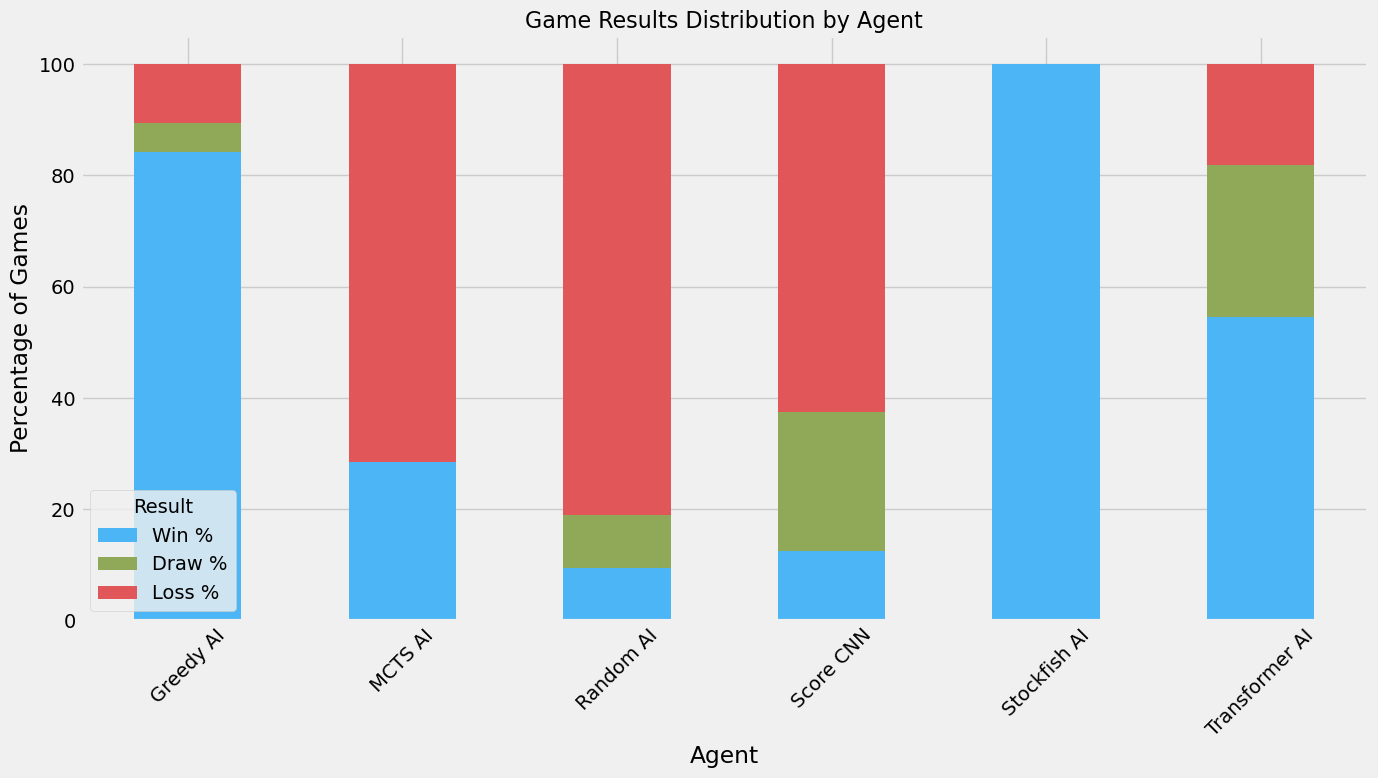
\includegraphics[width=0.45\textwidth]{fig/win_rates.png}
    \caption{Win-Rates for different models against each other.}
    \label{fig:win_rates}
\end{figure}

\begin{figure}[H]
    \centering
    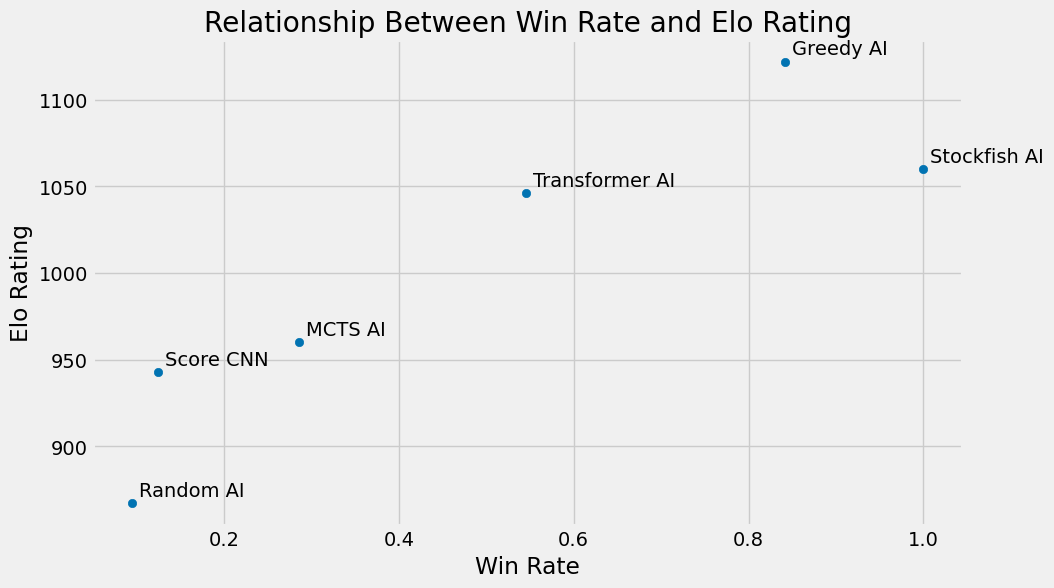
\includegraphics[width=0.45\textwidth]{fig/winrate_elo.png}
    \caption{Relationsship between Win Rate and Elo.}
    \label{fig:win_rates}
\end{figure}

\noindent Our evaluation revealed Stockfish AI as the strongest performing agent, consistently achieving wins in nearly all matches, underscoring its well-optimized heuristic evaluation and extensive tree search capabilities.

The Greedy AI, utilizing Alpha-Beta pruning with a handcrafted evaluation function, showed strong performance, winning most games and losing only a small fraction. Despite efficiency at moderate search depths, computational costs increased significantly with deeper exploration, occasionally leading to repetitive moves and draws.

The Transformer-based agent demonstrated promising results, securing numerous wins and draws, reflecting effective capture of global board relationships and strategic contexts through attention mechanisms. Nevertheless, it still experienced occasional losses, indicating room for improvement in generalization.

Monte Carlo Tree Search (MCTS), despite probabilistic exploration and nuanced decision-making, underperformed compared to the Greedy AI. Limited performance primarily resulted from the constraints of its evaluation function and inherent challenges applying Monte Carlo methods effectively to chess.

The CNN-based Score CNN exhibited modest success, achieving some wins and numerous draws but often losing due to generalization issues. Its key shortcomings included spatial invariance conflicts, inability to manage global positional relationships, frequent overfitting, and inability to capture sequential dependencies.

The Random AI consistently performed poorly, losing nearly all games, as expected from its random move selection strategy.

Q-Learning realistically faces significant challenges due to the extensive state-action space in chess but could benefit from function approximation methods to improve feasibility. TD-Learning combined with deep neural networks might provide effective learning through temporal experiences, potentially enhancing strategic evaluation.

Overall, our modular framework facilitated straightforward integration of diverse agent models, configurable game parameters (e.g., time controls, starting positions), a robust simulation environment, and efficient metrics analysis. The user-friendly frontend supports multiple gameplay modes (player vs. player, AI vs. player, AI vs. AI).

Nonetheless, some limitations persist:
\begin{enumerate}
    \item \textbf{Computational Efficiency}: Sophisticated models (MCTS, Transformers, CNNs) require significant computational resources, limiting real-time applications.
    \item \textbf{Training Data Quality}: Deep learning methods depend heavily on data quality and quantity.
    \item \textbf{Exploration-Exploitation Balance}: Achieving an optimal balance remains challenging, particularly for MCTS.
    \item \textbf{Time Constraints}: Limited decision-making time frequently results in suboptimal moves in complex positions.
\end{enumerate}


\section{Conclusions}
\label{sec:conclusions}
\noindent In this project, we developed a modular framework for implementing, testing, and analyzing various chess-playing agents using traditional search techniques, reinforcement learning, and deep neural networks. Our findings underscore the effectiveness of heuristic-driven methods, with Stockfish AI and Greedy AI demonstrating robust performance due to their efficient search strategies and handcrafted evaluation functions.

Transformer-based models showed significant promise, effectively leveraging attention mechanisms to capture global positional contexts. In contrast, the CNN-based approach encountered generalization issues, highlighting challenges specific to spatial invariance and sequential dependencies in chess.

Critical insights emerged regarding the balance between computational efficiency and playing strength, highlighting practical constraints faced by sophisticated algorithms such as MCTS and deep neural networks. The modularity of our framework enabled rapid experimentation and facilitated direct comparison of diverse methodologies.

Future research could focus on hybrid models combining strengths of heuristic search and neural network-based approaches to enhance overall performance. Additionally, further optimizing these methods for computational efficiency could significantly improve real-time decision-making capabilities.


\newpage

\bibliography{references}

\newpage
%\section*{Appendix}
%\label{sec:appendix}

%\subsection*{Model Architecture Details}

%\subsubsection*{MCTS Node Structure}
%In the MCTS algorithm, each node in the search tree represents a specific board position and stores essential information for decision-making. It maintains the current board state, a reference to its parent node, and the move that led to its creation. Additionally, the node keeps a list of child nodes representing possible future positions and tracks key statistics such as the number of wins and visits, which are crucial for guiding exploration and exploitation. To facilitate expansion, the node also maintains a list of untried moves that have not yet been explored in the search process.\\

%\subsubsection*{CNN Architecture}
% Encoder: ChessEmbedding`

%The schema represents the embedding module of a chess AI, which processes an input tensor of shape (b, 8, 8, 13); where 12 channels encode the chessboard using one-hot encoding for piece positions, and 1 channel represents the turn. The input first passes through a series of depthwise residual blocks that extract spatial and structural features from the board while preserving efficiency. In parallel, a heatmap extraction module applies convolution and Squeeze-and-Excitation (SE) attention and a sigmoid activation function to produce four specialized 8×8 feature maps, capturing positional importance. 


%\begin{figure}[H]
%    \centering
%    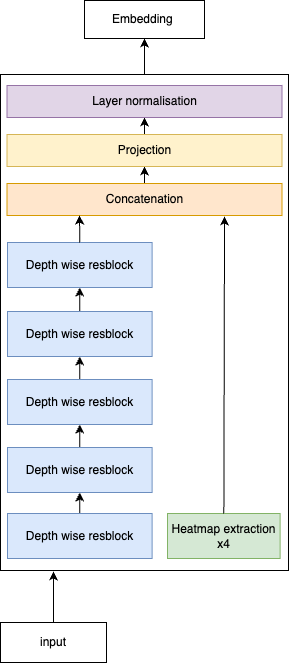
\includegraphics[width=0.3\textwidth]{CNN-embedding.drawio.png}
%    \caption{CNN Embedding Architecture}
%    \label{fig:cnn_embedding}
%\end{figure}

%The outputs from the residual blocks and heatmaps are then concatenated into a single tensor before undergoing a linear projection, reducing dimensionality while enhancing the feature representation. A layer normalization step ensures stable training and prevents feature scaling issues. The final output is a 768-dimensional embedding, which serves as the fundamental input for various downstream tasks, such as board evaluation, game generation, and move prediction.

\end{document}